\documentclass[paper=a4]{article}
\usepackage{ucs}
\usepackage[utf8x]{inputenc}
\usepackage[T1]{fontenc}
\PreloadUnicodePage{0}
\usepackage{xspace}
\usepackage{array}
\usepackage[hmargin=3.5cm,vmargin=2.7cm]{geometry} 
\usepackage{graphicx}
\usepackage{mathtools}

\renewcommand{\contentsname}{Innhold}
\title{Spillmanual}
\author{Team Dank}

\begin{document}
\author{Team Dank \\
Universitetet i Bergen \\
Informatikk}
\maketitle
\newpage
\tableofcontents
\newpage

\section{Introduksjon}
Dette er et spill tiltenkt datamaskiner der spillere kjemper om å overleve lengre enn sine motstandere. Det kan være opp til 4 spillere, men minimum 2. 
Spillet er et rundebasert 2D-platform strategi artilleri spill. Spillerne kan bevege seg i 30 sekunder for å posisjonere seg. 
Etter alle har posisjonert seg vil de ha muligheten til å sikte seg inn på fiender med våpen som skyter matvarer. 
Disse matvarene er melk, osv i skrivende stund, flere kan bli implementert i senere versjoner. % TODO
Når man har truffet en fiende, vil denne fienden legge på seg det antall kalorier matvaren inneholder. 
Dersom spilleren kommer over en grense kalorier vil spilleren tape, og er ute av spillet. Den som overlever til slutt vil vinne spillet.


\section{Systemkrav og installasjon}

\subsection{Systemkrav}
\begin{itemize}
	\item{Ikke mindre 1 GB RAM}
	\item{Windows Vista/Linux 2.6.12/Mac OS X 10.4 eller nyere}
	\item{50 MB ledig plass for installasjon}
	\item{Java 8}
	\item{Tastatur og mus}
	\item{TeamDank anbefaler deg å ha en prosessor (2005+) med klokkefrekvens på 1.6 GHz eller bedre}
\end{itemize}

\subsection{Installasjon}
Du må først sørge for at du har installert den nyeste versjonen av Java og \\
for å kunne spille FoodFeud må du laste ned $foodfeud.jar$ filen. \\
Deretter åpner du filen som vanlig for å starte spillet.  
\newpage

\section{Spillinstruksjoner og -regler}

\subsection{Kontroll}
Din primære spillinngangsenhet er tastaturet, og kan gjøre følgende:
\begin{itemize}
	\item{Du styrer din spiller med piltastene eller $A$ og $D$, du kan hoppe ved å trykke pil opp eller $W$}
	\item{For å kunne gå opp mange av bakkene må du hoppe samtidig som du går oppover}
	\item{For at du skal være ferdig med din tur må du trykke på $space$}
	\item{Du kan pause spillet ved å gå til pausemenyen ved å trykke på tastaturknappen $ESC$, eller gå ut av spillet}
	\begin{itemize}
		\item{Å være på pausemenyen vil gi deg muligheten til å fortsette eller avslutte spillet.}
	\end{itemize}
\end{itemize}

\subsection{Object-interaksjon}
Det er forskjellige matvarer som blir brukt som skudd i FoodFeud, skaden blir bestemt av antall kalorier matvaren inneholder. Noen eksempler er:
\\
{\renewcommand\labelitemi{}
\begin{itemize}
	\item 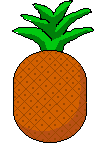
\includegraphics[scale = 0.3]{images/Ananas.png} \textbf{Ananas}
	\item 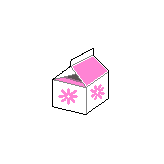
\includegraphics[scale = 0.4]{images/Melkekartong.png} \textbf{Melkekartong}
	\item 
\includegraphics[scale = 0.4]{images/Sushi.png} \textbf{Sushi}
	
\end{itemize}
}

\end{document}